
\subsection{Answers}
\begin{table}[htb]%
\begin{center}%
\caption{Q24: What, if any, alternatives are you investigating to indirectly call MPI or another communication layer by using another parallel language/library?}%
\label{tab:Q24-ans}%
\begin{tabular}{l|l|r}%
\hline%
Choice & Abbrv. & \# Answers \\%
\hline%
I am not investigating any alternatives. & No investigation & 402 (49.5\%) \\%
A framework or library using MPI. & Framework & 289 (35.6\%) \\%
{\small A PGAS language (UPC, Coarray Fortran, O$\cdots$} & PGAS & 142 (17.5\%) \\%
A Domain Specific Language (DSL). & DSL & 84 (10.3\%) \\%
{\small Low-level communication layer provided b$\cdots$} & LL comm & 52 (6.4\%) \\%
other & - & 26 (3.2\%) \\%
\hline%
\multicolumn{2}{c}{total} & 995 (812)\\%
\hline%
\end{tabular}%
\end{center}%
\end{table}%

\clearpage%
{\footnotesize\begin{landscape}%
\begin{longtable}[htb]{r|c|c|c|c|c|c|c|c|c|c}%
\caption{Q24: What, if any, alternatives are you investigating to indirectly call MPI or another communication layer by using another parallel language/library?}%
\label{tab:Q24-mans} \\%
\hline%
Multi-Answer & overall & FR & GR & IT & UK & eu & JP & RU & US & others \\
 \hline%
\endfirsthead%
\multicolumn{11}{r}{(continued from the previous page)}\\%
\hline%
Multi-Answer & overall & FR & GR & IT & UK & eu & JP & RU & US & others \\
 \hline%
\endhead%
\hline%
(total) & 812 & 116 & 153 & 52 & 63 & 139 & 64 & 92 & 55 & 78 \\%
\hline%
\multicolumn{11}{r}{(continue to the next page)}\\%
\endfoot%
\hline%
(total) & 812 & 116 & 153 & 52 & 63 & 139 & 64 & 92 & 55 & 78 \\%
\hline%
\endlastfoot%
\hline%
{No investigation} & 394 & 51 & 84 & 30 & 28 & 71 & 20 & 46 & 22 & 42 \\%
{Framework} & 166 & 26 & 28 & 10 & 6 & 24 & 12 & 28 & 10 & 22 \\%
{PGAS} & 56 & 8 & 9 & 2 & 3 & 12 & 8 & 8 & 3 & 3 \\%
{Framework, PGAS} & 42 & 4 & 5 & 1 & 9 & 9 & 7 & 1 & 4 & 2 \\%
{Framework, DSL} & 26 & 5 & 3 & 0 & 6 & 5 & 3 & 3 & 1 & 0 \\%
{DSL} & 19 & 4 & 0 & 3 & 3 & 1 & 2 & 2 & 2 & 2 \\%
{LL comm} & 15 & 4 & 3 & 0 & 1 & 2 & 3 & 0 & 2 & 0 \\%
{Framework, LL comm} & 14 & 1 & 3 & 1 & 0 & 2 & 6 & 0 & 0 & 1 \\%
{Framework, PGAS, DSL} & 13 & 2 & 2 & 1 & 3 & 2 & 0 & 1 & 1 & 1 \\%
{PGAS, DSL} & 11 & 2 & 2 & 2 & 2 & 1 & 1 & 0 & 0 & 1 \\%
{Framework, No investigation} & 8 & 0 & 2 & 1 & 0 & 3 & 1 & 0 & 0 & 1 \\%
{Framework, PGAS, LL comm} & 6 & 0 & 1 & 0 & 0 & 1 & 0 & 1 & 2 & 1 \\%
{PGAS, LL comm} & 6 & 0 & 0 & 0 & 0 & 3 & 0 & 0 & 3 & 0 \\%
{Framework, PGAS, DSL, LL comm} & 4 & 1 & 0 & 0 & 0 & 0 & 0 & 0 & 2 & 1 \\%
{DSL, LL comm} & 3 & 2 & 0 & 0 & 1 & 0 & 0 & 0 & 0 & 0 \\%
{GASPI} & 2 & 0 & 2 & 0 & 0 & 0 & 0 & 0 & 0 & 0 \\%
{Framework, DSL, LL comm} & 2 & 0 & 0 & 0 & 0 & 1 & 0 & 0 & 0 & 1 \\%
{Framework, PGAS, HPX with MPI parcelport} & 1 & 0 & 1 & 0 & 0 & 0 & 0 & 0 & 0 & 0 \\%
{DSL, gaspi} & 1 & 1 & 0 & 0 & 0 & 0 & 0 & 0 & 0 & 0 \\%
{Global Arrays} & 1 & 0 & 1 & 0 & 0 & 0 & 0 & 0 & 0 & 0 \\%
{OpenSHMEM only} & 1 & 0 & 0 & 0 & 1 & 0 & 0 & 0 & 0 & 0 \\%
{PGAS, DSL, HPX} & 1 & 0 & 0 & 0 & 0 & 1 & 0 & 0 & 0 & 0 \\%
{Framework, write my own library} & 1 & 0 & 0 & 0 & 0 & 0 & 0 & 0 & 1 & 0 \\%
{Framework, Dynamic runtime system that MPI usage to provide asynchronous execution} & 1 & 0 & 0 & 0 & 0 & 0 & 0 & 0 & 1 & 0 \\%
{I rely on the work of master expert developers} & 1 & 0 & 0 & 1 & 0 & 0 & 0 & 0 & 0 & 0 \\%
{Framework, NCCL} & 1 & 0 & 0 & 0 & 0 & 0 & 0 & 1 & 0 & 0 \\%
{LL comm, GASPI} & 1 & 0 & 1 & 0 & 0 & 0 & 0 & 0 & 0 & 0 \\%
{Framework, DSL, Task runtimes such as starpu} & 1 & 1 & 0 & 0 & 0 & 0 & 0 & 0 & 0 & 0 \\%
{PGAS, DSL, LL comm} & 1 & 0 & 1 & 0 & 0 & 0 & 0 & 0 & 0 & 0 \\%
{Trilinos} & 1 & 0 & 1 & 0 & 0 & 0 & 0 & 0 & 0 & 0 \\%
{Hpx} & 1 & 0 & 0 & 0 & 0 & 0 & 0 & 0 & 1 & 0 \\%
{Task-based runtime systems} & 1 & 1 & 0 & 0 & 0 & 0 & 0 & 0 & 0 & 0 \\%
{Framework, HDF5} & 1 & 0 & 1 & 0 & 0 & 0 & 0 & 0 & 0 & 0 \\%
{Framework, Matlab Distributed Computing Functionality} & 1 & 0 & 1 & 0 & 0 & 0 & 0 & 0 & 0 & 0 \\%
{Framework, runtime} & 1 & 1 & 0 & 0 & 0 & 0 & 0 & 0 & 0 & 0 \\%
{PGAS, DSL, I made my own DSL} & 1 & 0 & 0 & 0 & 0 & 1 & 0 & 0 & 0 & 0 \\%
{runtime system, StarPU, newmadeleine} & 1 & 1 & 0 & 0 & 0 & 0 & 0 & 0 & 0 & 0 \\%
{DSL, NCCL} & 1 & 0 & 0 & 0 & 0 & 0 & 1 & 0 & 0 & 0 \\%
{GASPI / GPI2} & 1 & 0 & 1 & 0 & 0 & 0 & 0 & 0 & 0 & 0 \\%
{(dask)} & 1 & 1 & 0 & 0 & 0 & 0 & 0 & 0 & 0 & 0 \\%
{DVM, NORMA} & 1 & 0 & 0 & 0 & 0 & 0 & 0 & 1 & 0 & 0 \\%
{HPX} & 1 & 0 & 1 & 0 & 0 & 0 & 0 & 0 & 0 & 0 \\%
\hline%
\end{longtable}%
\end{landscape}}%
\clearpage%


\subsection{List of other answers}
\begin{itemize}
\item Europe:France: (dask)
\item Europe:France: Task runtimes such as starpu
\item Europe:France: Task-based runtime systems
\item Europe:France: gaspi
\item Europe:France: runtime
\item Europe:France: runtime system, StarPU, newmadeleine
\item Europe:Germany: GASPI
\item Europe:Germany: GASPI
\item Europe:Germany: GASPI
\item Europe:Germany: GASPI / GPI2
\item Europe:Germany: Global Arrays
\item Europe:Germany: HDF5
\item Europe:Germany: HPX
\item Europe:Germany: HPX with MPI parcelport
\item Europe:Germany: Matlab Distributed Computing Functionality
\item Europe:Germany: Trilinos
\item Europe:Italy: I rely on the work of master expert developers
\item Europe:UK: OpenSHMEM only
\item Europe:others: HPX
\item Europe:others: I made my own DSL
\item Japan: NCCL
\item Russia: DVM, NORMA
\item Russia: NCCL
\item USA: Dynamic runtime system that MPI usage to provide asynchronous execution
\item USA: Hpx
\item USA: write my own library

\end{itemize}

The main way to access MPI is done by calling the library directly (41\%). If this is
not the case the most current way  of alternatively calling MPI is through
libraries (28\%). Language approaches, such as PGAS or DSL are less used methods
(resp. 14.1\% and 8.3\%).  This means that MPI is mostly seen as a way to program
parallel application and less an environment to be used by runtime systems or
languages.  

\begin{figure}[htb]
\begin{center}
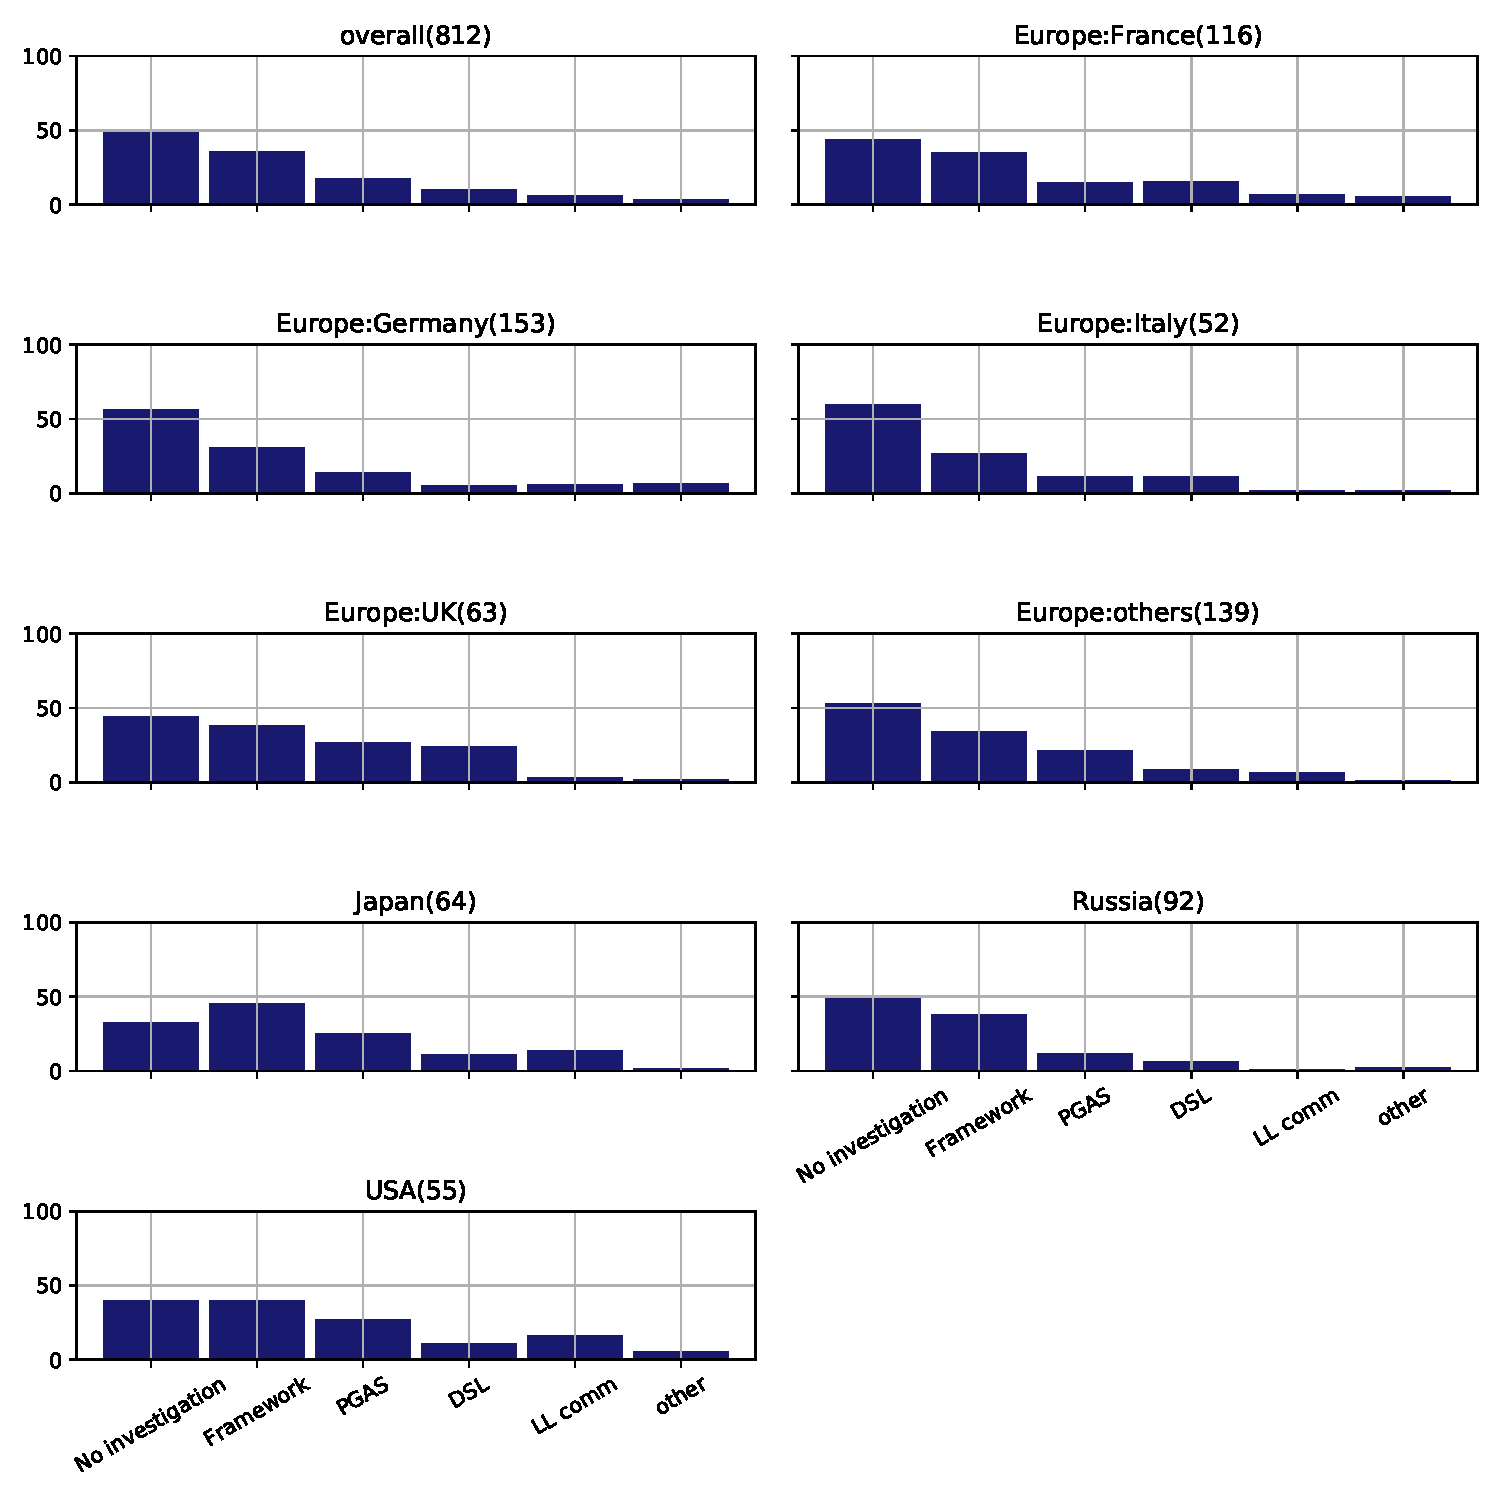
\includegraphics[width=10cm]{../pdfs/Q24.pdf}
\caption{Simple analysis: Q24}
\label{fig:Q24}
\end{center}
\end{figure}

\begin{figure}[htb]
\begin{center}
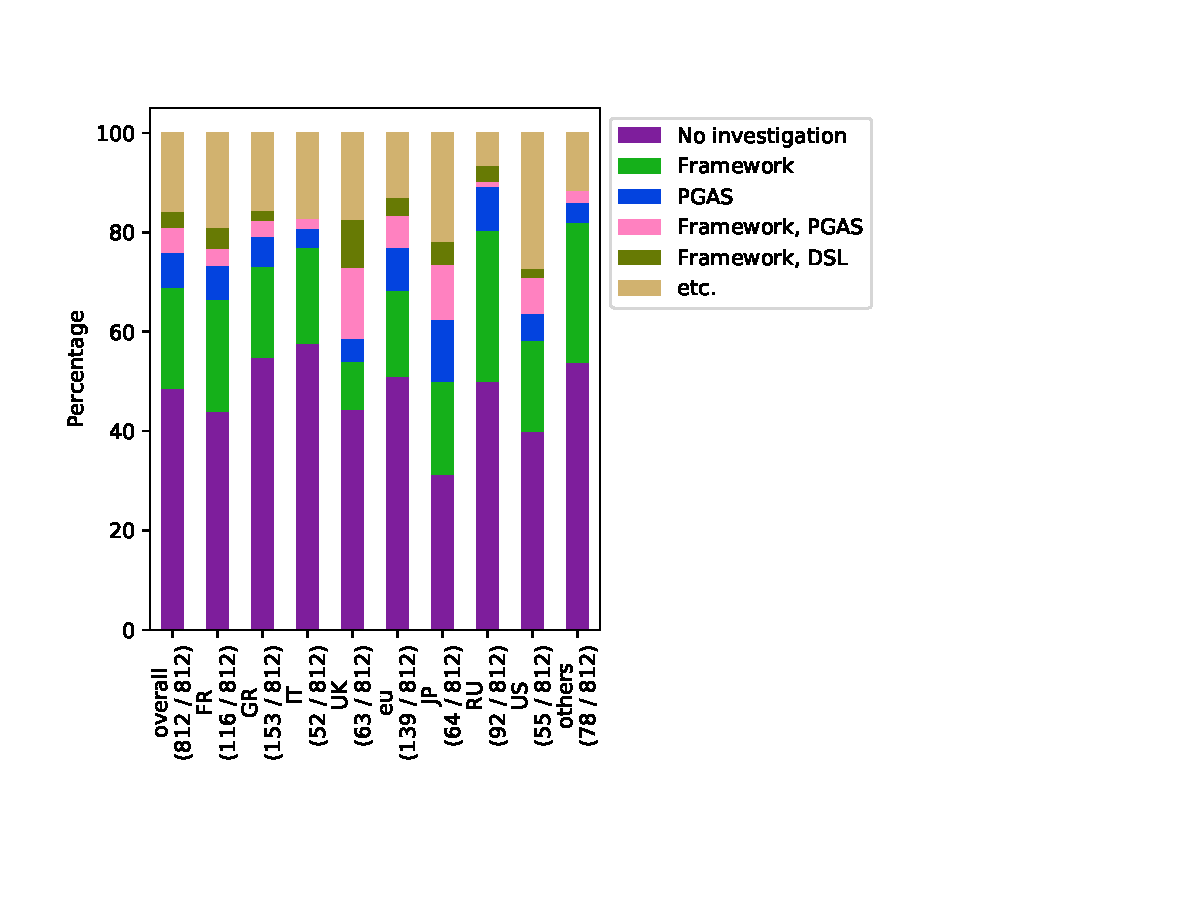
\includegraphics[width=14cm]{../pdfs/Q24-mans.pdf}
\caption{Multiple Answers: Q24}
\label{fig:Q24-mans}
\end{center}
\end{figure}

A fair amount of people are investigating frameworks of libraries
and/or PGAS languages as alternatives of MPI.  UK has the higest
percentage of investigating DSL. In contrast, Germany has the lowest
percentage of investigating DSL. 
